\documentclass{article}

\usepackage{cancel}
\usepackage{amsmath}
\usepackage[includehead,nomarginpar]{geometry}
\usepackage{graphicx}
\usepackage{amsfonts} 
\usepackage{verbatim}
\usepackage{mathrsfs}  
\usepackage{lmodern}
\usepackage{braket}
\usepackage{bookmark}
\usepackage{fancyhdr}
\usepackage{romanbarpagenumber}
\usepackage{minted}
%\usepackage{subfig}
\usepackage[italian]{babel}
%\usepackage{float}
%\usepackage{wrapfig}
%\usepackage[export]{adjustbox}
\allowdisplaybreaks

\setlength{\headheight}{12.0pt}
\addtolength{\topmargin}{-12.0pt}
\graphicspath{ {../Immagini/} }

\hypersetup{
    colorlinks=true,
    linkcolor=black,
}

\newsavebox{\tempbox} %{\raisebox{\dimexpr.5\ht\tempbox-.5\height\relax}}


\makeatother

\numberwithin{equation}{subsection}
\newcommand{\tageq}{\tag{\stepcounter{equation}\theequation}}
\AtBeginDocument{%
  \renewcommand{\figurename}{Fig.}
}
\fancypagestyle{link}{\fancyhf{}\renewcommand{\headrulewidth}{0pt}\fancyfoot[C]{Sorgente del file LaTeX disponibile al seguente link: \url{https://github.com/00Darxk/Reti-di-Calcolatori/}}}

\begin{document}

\title{%
    \textbf{Reti di Calcolatori}  \\ 
    \large Appunti delle Lezioni di Reti di Calcolatori \\
    \textit{Anno Accademico: 2024/25}}
\author{\textit{Giacomo Sturm}}
\date{\textit{Dipartimento di Ingegneria Civile, Informatica e delle Tecnologie Aeronautiche \\
Università degli Studi ``Roma Tre"}}

\maketitle
\thispagestyle{link}

\clearpage


\pagestyle{fancy}
\fancyhead{}\fancyfoot{}
\fancyhead[C]{\textit{Reti di Calcolatori - Università degli Studi ``Roma Tre"}}
\fancyfoot[C]{\thepage}
\pagenumbering{Roman}

\tableofcontents

\clearpage
\pagenumbering{arabic}

\section{Esercitazione 23/10/24}

\subsection{Rete Bridge con Cicli}

Si considera una rete locale IEEE 802.3 di topologia seguente:

%% TODO img topologia esercizio

Sono presenti due repeater R, e due computer A e B. Le connessioni avvengono solo su cavi utp, ``Unshielded Twisted Pair'', si suppone che questi 
bridge numerati 1 e 2, non siano in grado di realizzare lo spanning tree. Quindi tutta la rete, compreso il ciclo, è attiva. Si suppone che tutte 
le porte dei bridge siano pienamente attive. 
Si suppone che i bridge siano appena stati accesi, quindi i loro filtering database siano vuoti. 

Il primo evento in questa rete locale è l'invio di un pacchetto da A e B. 

\subsubsection*{Domanda 1}

Determinare quanti pacchetti circolano nella rete dopo l'invio del singolo pacchetto. 
Questo pacchetto \verb|(A->B)| arriva ad entrambi i bridge \verb|bridge 1| e \verb|bridge 2|, che hanno un filtering database vuoto, per cui lo mandano su tutte le 
porte attive. Poiché il repeater può inviare ricevere un pacchetto alla volta si considera che il pacchetto del primo bridge arrivi per primo al repeater, nella 
contesa del dominio di collisione. Si considerano i due pacchetti copiati dai due bridge \verb|(A->B)'|, il primo, e \verb|(A->B)'|, il secondo. 
Ma il repeater invia il pacchetto ricevuto su tutte le direzioni, quindi oltre ad arrivare a B, arriva anche alla porta destra dell'altro bridge, che invia la sua copia 
del pacchetto dalla porta sinistra. Questo pacchetto incontra il repeater della sotto-rete A e viene ripetuto su tutte le porte del repeater. Quindi questo pacchetto 
oltre a raggiungere A viene inviato sulla porta sinistra dell'altro bridge, e si ripete la sequenza, per entrambi i bridge. 

Quindi in questa situazione le copie del pacchetto \verb|(A->B)'| viene inviato continuamente in un ciclo antiorario, mentre \verb|(A->B)''| segue il percorso 
orario. 


\subsubsection*{Domanda 2}

Determinare cosa succeeded al filtering database di \verb|bridge 1| e \verb|bridge 2|. 
Ogni volta che il pacchetto copiato raggiunge un bridge, considera la porta da cui è arrivato la nuova posizione della stazione A, così per entrambi i bridge. 
Quindi la sua posizione nel filtering database cambia continuamente. 

\subsubsection*{Domanda 3}

Determinare il comportamento dei bridge all'invio di un pacchetto \verb|(B->A)|. Se il pacchetto arriva ad entrambi i bridge quando la stazione A si trova nel 
filtering database sulla porta destra, il pacchetto non viene inviato ad A. Se solo uno presenta la stazione A alla porta sinistra, una singola copia raggiunge A. 
Se entrambi presentano la stazione A alla porta sinistra, questa riceve due volte il pacchetto. 


Dati questi problemi non si accetta di avere un ciclo in una rete neanche per un tempo transitorio, poiché può saturare la rete ed impedire ai pacchetti necessari a 
passare. Gli algoritmi per determinare lo spanning tree sono molto conservativi, e prima di effettuare l'algoritmo interrompono il transito di tutti i pacchetti. 

\subsection{Effetto dlo Store \& Forward sulla Latenza}

Si considera una rete mostrata nella figura seguente, dove A e B sono computer e S1 e S2 sono switch. Dove i cavi ethernet sono utp, ed il ritardo di propagazione 
è trascurabile. Si suppone che le schede di rete utilizzate sono tutte a 10 Mb/s. 

Questo disegno mostra cosa avviene sulla rete mentre è in funzione, rispetto al tempo:

\begin{figure}[H]%
    \centering%
    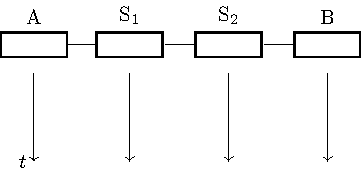
\includegraphics{effetto_store_forward.pdf}%
\end{figure}

Il computer deve spedire un file di 100000 bit a B, suddividendolo in 100 pacchetti. Si suppone ch eil trasferimento inizi all'istante $t=0$, e si suppone di trascurare 
gli header e l'IPG. Si suppone che la rete sia a completa disposizione del trasferimento dei file, che gli switch non operino in modalità ``cut-through''. Si suppone che non 
siano utilizzati riscontri di alcun tipo. 

\subsubsection*{Domanda 1}

Completa il diagramma temporale riportato al di sotto della figura con la rete, mostrando la sequenza dell'invio dei pacchetti dai vari componenti:

\begin{figure}[H]%
    \centering%
    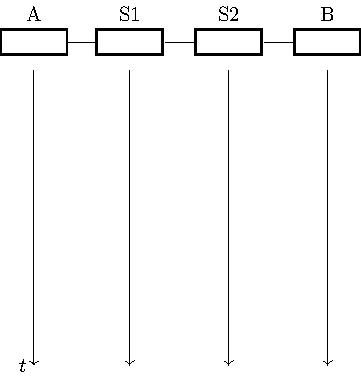
\includegraphics{effetto_store_forward_domanda_1.pdf}%
\end{figure}

Ad ogni istante lo switch ha un pacchetto in ricezione su una porta, ed un pacchetto in trasmissione sulla seconda porta. 

Per inviare un singolo pacchetto sulla rete si impiega un tempo $t_i$:

\begin{equation}
    t_i=\displaystyle\frac{100000 \mathrm{bit}/100\mathrm{pk}}{10^7 \mathrm{bit/s}}=10^{-4}\mathrm{s/pk}
\end{equation}

In caso il ritardo non sia trascurabile, ogni segmento viene traslato verso il basso di questo ritardo. 

\subsubsection*{Domanda 2}

In quale istante tutti i bit sono arrivati a B:


Il primo pacchetto viene ricevuto completamente ad un tempo $3t_i$, poiché deve passare attraverso tre spazi intermedi, quindi l'ultimo pacchetto 
viene ricevuto completamente all'istante $102t_i$. 

\subsubsection*{Domanda 3}

Determinare una formula generale per risolvere ogni problema di questo tipo con $n$ pacchetti ed $m$ switch. 

%% TODO img disegno e risposta

\subsubsection*{Domanda 4}

Determinare una formula generale che tenga conto di ritardi sul primo, sul secondo, o sul terzo filo. 

%% TODO img disegno e risposta

\subsubsection*{Domanda 5}

Si suppone di poter aumentare la connessione ad una banda di 100 Mb/s, ma questo aumento è possibile solo su uno dei tre fili, utilizzando 
una doppia scheda su di un filo. 

%% TODO img disegno e risposta

\subsection{Learning nei Bridge}

\subsubsection*{Domanda 1}

Si considera un bridge B1 con quattro porte \verb|eth0|, \verb|eth1|, \verb|eth2| e \verb|eth3|, a cui sono collegati quattro computer A, B, C, D. Nella rete transitano 
cinque pacchetti seguenti, inviati dopo che il precedente è giunto a destinazione: 
\begin{itemize}
    \item t$_1$: \verb|(a->b)|;
    \item t$_2$: \verb|(b->a)|;
    \item t$_3$: \verb|(c->d)|;
    \item t$_4$: \verb|(c->d)|;
    \item t$_5$: \verb|(d->a)|;
\end{itemize}

Descrivere il contenuto del filtering database di B1, dopo ciascun pacchetto, e specificare le porzioni di rete in cui i diversi pacchetti sono visibili. 

Il pacchetto t$_1$ viene ricevuto dalla porta \verb|eth0|, quindi viene assegnata ad A nel filtering database, e viene inviato su tutte le altre le porte. 
Il pacchetto t$_2$ viene ricevuto dalla porta \verb|eth1|, questa porta viene associata al computer B, e sapendo dove si trova A, lo invia solamente sulla porta \verb|eth0|.
I pacchetti t$_3$ e t$_4$ effettuano un procedimento analogo a t$_1$ e t$_2$, sulle porte \verb|eth2| e \verb|eth3|. 
All'arrivo del pacchetto t$_5$, il bridge conosce l'intera topologia della rete. 

Ma il filtering database non è statico, e viene dimenticato in intervalli di tempo prestabiliti, oppure se uno dei computer viene connesso ad un'altra porta 
e ne riceve un pacchetto. Quindi se uno di questi pacchetti arriva dopo che è stato resettato il filtering database, ricomincia il processo di learning. 

\subsubsection*{Domanda 2}

Si considera la seguente topologia di rete ad albero, con tre bridge B1, B2, e B3, e tre computer A, B e C. 

%% TODO 

\subsubsection*{Domanda 3}

%% TODO 


\end{document}